\documentclass[10pt,tikz]{standalone}

\ifstandalone%
\usepackage{import}%
\import{../../configuration/}{comon_packages.tex}%
\import{../../configuration/}{variables.tex}%
\import{../../configuration/}{conftikz.tex}%
\import{../../configuration/}{custom_config.tex}%
\fi

\begin{document}
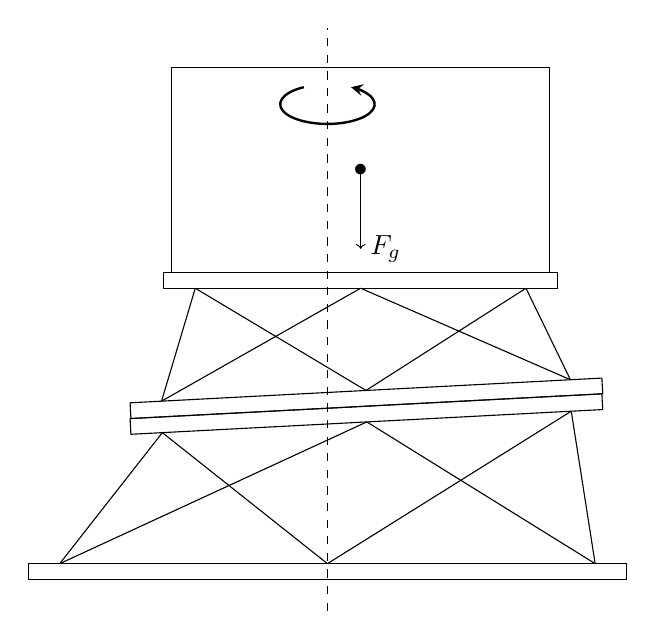
\begin{tikzpicture}
  \newcommand{\AxisRotator}[1][rotate=0]{%
    \tikz [x=0.25cm,y=0.60cm,line width=.2ex,-stealth,#1] \draw (0,0) arc (-150:150:1 and 1);%
  }

  % Parameters definitions
  \def\baseh{0.2} % Height of the base
  \def\naceh{0.2} % Height of the nacelle
  \def\baser{3.8} % Radius of the base
  \def\nacer{3.0} % Radius of the nacelle

  \def\armr{0.2} % Radius of the arms
  \def\basearmborder{0.2}
  \def\nacearmborder{0.2}

  \def\xnace{0.5} % X position of the nacelle
  \def\ynace{2.0} % Y position of the nacelle
  \def\anace{3.0} % Angle of the nacelle

  \def\xbase{0.0} % X position of the base
  \def\ybase{0.0} % Y position of the base
  \def\abase{0.0} % Angle of the base

  % Hexapod1
  \begin{scope}[shift={(\xbase, \ybase)}, rotate=\abase]
    % Base
    \draw[] (-\baser, 0) rectangle (\baser, \baseh);

    \coordinate[] (armbasel) at (-\baser+\basearmborder+\armr, \baseh);
    \coordinate[] (armbasec) at (0, \baseh);
    \coordinate[] (armbaser) at (\baser-\basearmborder-\armr, \baseh);

    % Nacelle1
    \begin{scope}[shift={(\xnace, \ynace)}, rotate=\anace]
      \draw[] (-\nacer, 0) rectangle (\nacer, \naceh);
      \coordinate[] (armnacel) at (-\nacer+\nacearmborder+\armr, 0);
      \coordinate[] (armnacec) at (0, 0);
      \coordinate[] (armnacer) at (\nacer-\nacearmborder-\armr, 0);
    \end{scope}
    % Nacelle1 END

    \draw[] (armbasec) -- (armnacer);
    \draw[] (armbasec) -- (armnacel);
    \draw[] (armbasel) -- (armnacel);
    \draw[] (armbasel) -- (armnacec);
    \draw[] (armbaser) -- (armnacec);
    \draw[] (armbaser) -- (armnacer);

    % Hexapod2
    \begin{scope}[shift={(\xnace, \ynace+\baseh)}, rotate=\anace]
      \def\baser{3.0} % Radius of the nacelle
      \def\nacer{2.5} % Radius of the nacelle
      \def\xnace{0.0} % X position of the nacelle
      \def\ynace{1.5} % Y position of the nacelle

      \def\anace{-3.0} % Angle of the nacelle

      % Base
      \draw[] (-\baser, 0) rectangle (\baser, \baseh);

      \coordinate[] (armbasel) at (-\baser+\basearmborder+\armr, \baseh);
      \coordinate[] (armbasec) at (0, \baseh);
      \coordinate[] (armbaser) at (\baser-\basearmborder-\armr, \baseh);

      % Nacelle2
      \begin{scope}[shift={(\xnace, \ynace)}, rotate=\anace]
        \draw[] (-\nacer, 0) rectangle (\nacer, \naceh);
        \coordinate[] (armnacel) at (-\nacer+\nacearmborder+\armr, 0);
        \coordinate[] (armnacec) at (0, 0);
        \coordinate[] (armnacer) at (\nacer-\nacearmborder-\armr, 0);

        \draw[] (armbasec) -- (armnacer);
        \draw[] (armbasec) -- (armnacel);
        \draw[] (armbasel) -- (armnacel);
        \draw[] (armbasel) -- (armnacec);
        \draw[] (armbaser) -- (armnacec);
        \draw[] (armbaser) -- (armnacer);

        % Sample
        \begin{scope}[shift={(0, \naceh)}]
          \def\samph{2.6} % Height of the sample
          \def\sampr{2.4} % Radius of the sample
          \draw[] (-\sampr, 0) rectangle (\sampr, \samph);

          \coordinate[] (massc) at (0, 0.5*\samph);
          \draw[->] (massc) node[]{$\bullet$} -- ++(0,-1) node[right]{$F_g$};
        \end{scope}
        % Sample END
      \end{scope}
      % Nacelle2 END
    \end{scope}
    % Hexapod2 END
  \end{scope}
  % Hexapod1 END

  \draw[dashed] (0, -0.4) -- (0, 7);
  \node[] at (0, 6) {\AxisRotator[rotate=-90]};
\end{tikzpicture}
\end{document}

